\documentclass[10pt,twocolumn]{article}
\usepackage[margin=0.9in]{geometry}
\usepackage{graphicx}

\title{\large{Spectral Clustring Based on Local PCA with Application to Hand-written Digit Separation}}
\author{
    Yu, Guangting\thanks{Quantitative Finance \& Risk Management, Department of Mathematics} \\
    \small{\texttt{yugtmath@umich.edu}}
    \and
    Jia, Guo\thanks{Applied \& Interdisciplinary Math Ph.D., Department of Mathematics} \\
    \texttt{guojia@umich.edu}
    \and
    Tsukamoto, Masaya\thanks{Quantitative Finance \& Risk Management, Department of Mathematics} \\
    \texttt{masayats@umich.edu}
    \and
    Wang, Zihan\thanks{Space Science Ph.D., Department of Climate and Space Sciences and Engineering} \\
    \texttt{wzihan@umich.edu}
}


\begin{document}
\maketitle
\subsection*{Problem statement}
In hand-written digit recognition, if the digits are connected, (like `2' and `0' in Figure \ref{fig1}), there is no chance for the classifier to output the correct result.
\begin{figure}[htbp]
\centering

\includegraphics[width=0.1\textwidth]{connected-digits.png}
\hspace{1em}
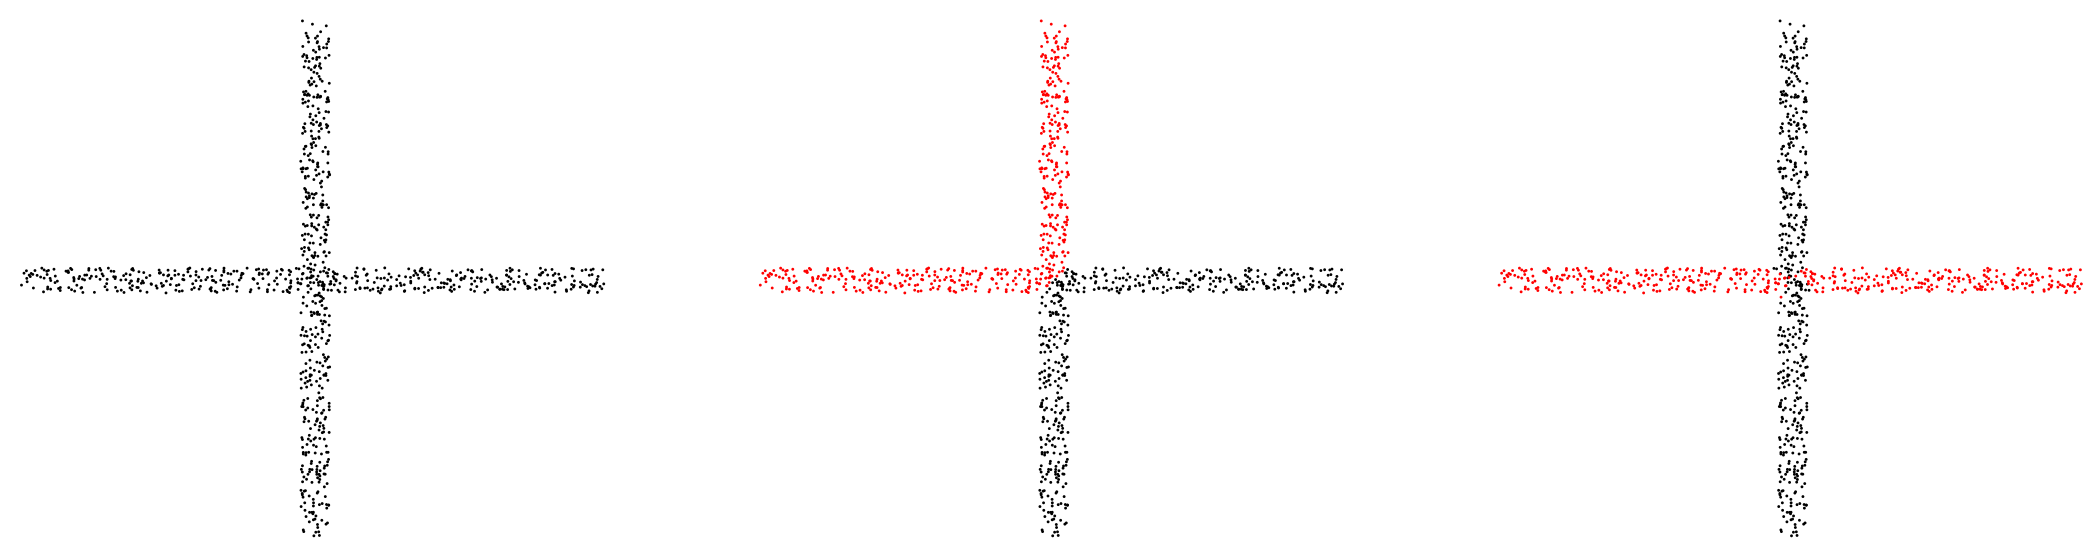
\includegraphics[width=0.3\textwidth]{effect.png}
\label{fig1}
\caption{(1) Connected digits, (2) sample pixels (3) spectral clustering by Ng. et al (2002), (4) spectral clustering by local PCA}
\end{figure}
So we want to separate the connected digits apart.
\subsection*{Motivation}

\subsection*{Papers to focus on}
\subsection*{Methods to be compared}
\subsection*{Data sets}
\subsection*{Group member roles}
\end{document}